\let\negmedspace\undefined
\let\negthickspace\undefined
\documentclass[journal]{IEEEtran}
\usepackage[a5paper, margin=10mm, onecolumn]{geometry}
\usepackage{lmodern} % Ensure lmodern is loaded for pdflatex
\usepackage{tfrupee} % Include tfrupee package

\setlength{\headheight}{1cm} % Set the height of the header box
\setlength{\headsep}{0mm}     % Set the distance between the header box and the top of the text

\usepackage{gvv-book}
\usepackage{gvv}
\usepackage{cite}
\usepackage{amsmath,amssymb,amsfonts,amsthm}
\usepackage{algorithmic}
\usepackage{graphicx}
\usepackage{textcomp}
\usepackage{xcolor}
\usepackage{txfonts}
\usepackage{listings}
\usepackage{enumitem}
\usepackage{mathtools}
\usepackage{gensymb}
\usepackage{comment}
\usepackage[breaklinks=true]{hyperref}
\usepackage{tkz-euclide} 
\usepackage{listings}
\def\inputGnumericTable{}                                 
\usepackage[latin1]{inputenc}                                
\usepackage{color}                                            
\usepackage{array}                                            
\usepackage{longtable}                                       
\usepackage{calc}                                             
\usepackage{multirow}                                         
\usepackage{hhline}                                           
\usepackage{ifthen}                                           
\usepackage{lscape}

\begin{document}
	
	\bibliographystyle{IEEEtran}
	\vspace{3cm}
	
	\title{10.3.2.3.1}
	\author{EE24BTECH11030 - KEDARANANDA}
	% \maketitle
	% \newpage
	% \bigskip
	{\let\newpage\relax\maketitle}
	
	\renewcommand{\thefigure}{\theenumi}
	\renewcommand{\thetable}{\theenumi}
	\setlength{\intextsep}{10pt} % Space between text and floats
	
	\textbf{Question:}
	\newline
	On comparing the ratios $\frac{a_1}{a_2},\frac{b_1}{b_2} \text{and} \frac{c_1}{c_2}$, find out whether the following pair of linear equations are consistent, or inconsistent . 
	\begin{align}
		3x + 2y = 5 ; 2x - 3y = 7
	\end{align}
	\textbf{Theoritical Solution:}
	To determine whether the given pair of linear equations is consistent or inconsistent, we compare the ratios $\frac{a_1}{a_2}$, $\frac{b_1}{b_2}$, and $\frac{c_1}{c_2}$, where:
	
	\begin{align}
		a_1x + b_1y = c_1 \quad \text{and} \quad a_2x + b_2y = c_2
	\end{align}
	
	From the equations:
	\begin{align}
		3x + 2y = 5 \quad \text{and} \quad 2x - 3y = 7,
	\end{align}
	we identify:
	\begin{align}
		a_1 = 3, \, b_1 = 2, \, c_1 = 5, \, a_2 = 2, \, b_2 = -3, \, c_2 = 7.
	\end{align}
	
	Now calculate the ratios:
	\begin{align}
		\frac{a_1}{a_2} = \frac{3}{2}, \quad \frac{b_1}{b_2} = \frac{2}{-3}, \quad \frac{c_1}{c_2} = \frac{5}{7}.
	\end{align}
	
	Since:
	\begin{align}
		\frac{a_1}{a_2} \neq \frac{b_1}{b_2},
	\end{align}
	the given pair of equations is \textbf{consistent} and the lines represented by the equations are \textbf{intersecting}. Therefore, the system of equations has a unique solution.\\\\
	\textbf{Computational Solution:}
	\newline
	\section*{Solution using LU Factorization}
	
	Given the system of linear equations:
	\begin{align}
		3x + 2y &= 5, \label{eq1} \\
		2x - 3y &= 7. \label{eq2}
	\end{align}
	
	We rewrite the equations as:
	\begin{align}
		x_1 &= x, \\
		x_2 &= y,
	\end{align}
	giving the system:
	\begin{align}
		3x_1 + 2x_2 &= 5, \label{eq3} \\
		2x_1 - 3x_2 &= 7. \label{eq4}
	\end{align}
	
	\subsection*{Step 1: Convert to Matrix Form}
	We write the system as:
	\begin{align}
		A \mathbf{x} &= \mathbf{b},
	\end{align}
	where:
	\begin{align}
		A &= \begin{bmatrix} 3 & 2 \\ 2 & -3 \end{bmatrix}, \\
		\mathbf{x} &= \begin{bmatrix} x_1 \\ x_2 \end{bmatrix}, \\
		\mathbf{b} &= \begin{bmatrix} 5 \\ 7 \end{bmatrix}.
	\end{align}
	\subsection*{Step 2: LU factorization using update equaitons}
	Given a matrix $ \mathbf{A} $ of size $ n \times n $, LU decomposition is performed row by row and column by column. The update equations are as follows:\\
	\textbf{Step-by-Step Procedure:}\\
	1. Initialization: 
	- Start by initializing $ \mathbf{L} $ as the identity matrix $ \mathbf{L} = \mathbf{I} $ and $ \mathbf{U} $ as a copy of $ \mathbf{A} $.
	
	2. Iterative Update:
	- For each pivot $ k = 1, 2, \ldots, n $:
	- Compute the entries of $ U $ using the first update equation.
	- Compute the entries of $ L $ using the second update equation.
	
	3. Result:
	- After completing the iterations, the matrix $ \mathbf{A} $ is decomposed into $ \mathbf{L} \cdot \mathbf{U} $, where $ \mathbf{L} $ is a lower triangular matrix with ones on the diagonal, and $ \mathbf{U} $ is an upper triangular matrix.
	
	
	
	\subsection*{1. Update for $ U_{k,j} $ (Entries of $ U $)}
	
	For each column $ j \geq k $, the entries of $ U $ in the $ k $-th row are updated as:
	\[
	U_{k,j} = A_{k,j} - \sum_{m=1}^{k-1} L_{k,m} \cdot U_{m,j}, \quad \text{for } j \geq k.
	\]
	This equation computes the elements of the upper triangular matrix $ \mathbf{U} $ by eliminating the lower triangular portion of the matrix.
	
	\subsection*{2. Update for $ L_{i,k} $ (Entries of $ L $)}
	
	For each row $ i > k $, the entries of $ L $ in the $ k $-th column are updated as:
	\[
	L_{i,k} = \frac{1}{U_{k,k}} \left( A_{i,k} - \sum_{m=1}^{k-1} L_{i,m} \cdot U_{m,k} \right), \quad \text{for } i > k.
	\]
	This equation computes the elements of the lower triangular matrix $ \mathbf{L} $, where each entry in the column is determined by the values in the rows above it.\\
	\subsection*{Step 2: LU Factorization of Matrix A}
	We decompose $A$ as:
	\begin{align}
		A &= LU,
	\end{align}
	where $L$ is a lower triangular matrix and $U$ is an upper triangular matrix.
	by running the iteration code we get the L and U matrices :
	\begin{align}
		L &= \begin{bmatrix} 1 & 0 \\ \frac{2}{3} & 1 \end{bmatrix}, \\
		U &= \begin{bmatrix} 3 & 2 \\ 0 & -\frac{13}{3} \end{bmatrix}.
	\end{align}
	
	\subsection*{Step 3: Solve $L\mathbf{y} = \mathbf{b}$ (Forward Substitution)}
	We solve:
	\begin{align}
		L\mathbf{y} = \mathbf{b} \quad \text{or} \quad \begin{bmatrix} 1 & 0 \\ \frac{2}{3} & 1 \end{bmatrix} \begin{bmatrix} y_1 \\ y_2 \end{bmatrix} = \begin{bmatrix} 5 \\ 7 \end{bmatrix}.
	\end{align}
	From the first row:
	\begin{align}
		y_1 &= 5.
	\end{align}
	From the second row:
	\begin{align}
		\frac{2}{3} y_1 + y_2 &= 7 \quad \implies \quad \frac{2}{3} \cdot 5 + y_2 = 7 \quad \implies \quad y_2 = \frac{11}{3}.
	\end{align}
	
	Thus:
	\begin{align}
		\mathbf{y} &= \begin{bmatrix} 5 \\ \frac{11}{3} \end{bmatrix}.
	\end{align}
	
	\subsection*{Step 4: Solve $U\mathbf{x} = \mathbf{y}$ (Backward Substitution)}
	We solve:
	\begin{align}
		U\mathbf{x} = \mathbf{y} \quad \text{or} \quad \begin{bmatrix} 3 & 2 \\ 0 & -\frac{13}{3} \end{bmatrix} \begin{bmatrix} x_1 \\ x_2 \end{bmatrix} = \begin{bmatrix} 5 \\ \frac{11}{3} \end{bmatrix}.
	\end{align}
	From the second row:
	\begin{align}
		-\frac{13}{3} x_2 &= \frac{11}{3} \quad \implies \quad x_2 = -\frac{11}{13}.
	\end{align}
	From the first row:
	\begin{align}
		3x_1 + 2x_2 &= 5 \quad \implies \quad 3x_1 + 2 \left( -\frac{11}{13} \right) = 5, \\
		3x_1 - \frac{22}{13} &= 5 \quad \implies \quad 3x_1 = 5 + \frac{22}{13} = \frac{65}{13} + \frac{22}{13} = \frac{87}{13}, \\
		x_1 &= \frac{87}{39} = \frac{29}{13}.
	\end{align}
	
	Thus:
	\begin{align}
		\mathbf{x} &= \begin{bmatrix} x_1 \\ x_2 \end{bmatrix} = \begin{bmatrix} \frac{29}{13} \\ -\frac{11}{13} \end{bmatrix}.
	\end{align}
	
	\subsection*{Final Solution}
	The solution is:
	\begin{align}
		x &= \frac{29}{13}, \\
		y &= -\frac{11}{13}.
	\end{align}
	As we can clearly see that there is solution for the given lines these are consistent 
	\begin{figure}[!ht]
		\centering
		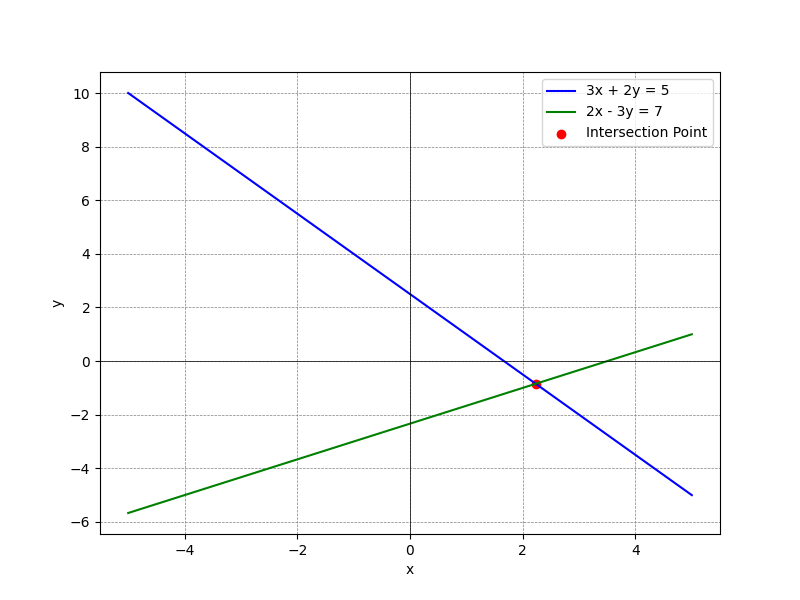
\includegraphics[width=\columnwidth]{figs/Fig.png}
		\caption{}
	\end{figure}
\end{document}